\section{Pilot Study}

As we see later in Section \ref{section:device-fingerprinting} the efficiency of the methods to clean and aggregate data not only depend on the noise and bias in the data itself but also on external factors such as, the configuration of the sensor in relation to the environment, the day of the week etc.
Thus the dataset captured in our initial experiments, though acts as a good starting point, cannot enable us to generalise our findings to all possible configurations.
This necessitates an even larger data collected over longer durations in challenging situations we usually find in real world conditions.
This was our primary motivation in conducting a pilot study collecting data at 5 locations across London.
The aim was to collect probe requests with information we found relevant in the initial experiments for every location surveyed for at least a full week so that we can understand any artifacts caused by the periodicity of the data.
We also wanted to collect data at all these locations in parallel for at least a week so that they can be compared to one other. 

\subsection{Methodology}

\begin{marginfigure}[2cm]
  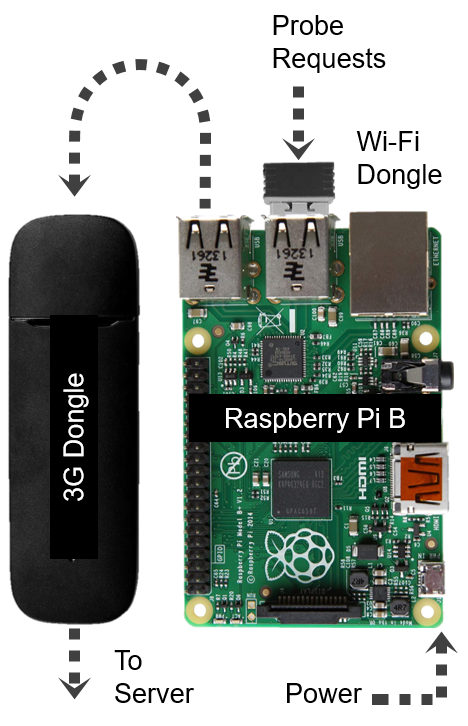
\includegraphics{images/pilot-hardware.png}
  \caption{Hardware setup used to collect data in the pilot studies.}
  \label{figure:collection:pilot:hardware}
\end{marginfigure}

The hardware setup for the sensors is illustrated in Figure \ref{figure:collection:pilot:hardware}.
It design of the hardware is not original as it is heavily influenced by the proprietary technology of the data partner for the Smart Street Sensor project albeit a much simpler form. 
The core of the hardware is the general purpose single board computer - Raspberry Pi Model B running Linux Operating system.
Two communication modules - 3G and Wi-Fi were connected to this machine via Universal Serial Bus interface.
3G modem was equipped with a SIM card which it uses to connect to the internet while the Wi-Fi modem is set to 'Monitor' mode.
The board takes power from an outlet and the software is pre installed with the operating system which resides in a Memory card.

The software used for the sensors consists of two parts - sensor software and server software.
The sensor software was written as a mix of Bash script and NodeJS.
Essentially these scripts use wireshark program to capture packets, parse them, anonymises the MAC address fields, adds the location information, encodes them into JavaScript Object Notation format and finally sends it to a server through Web-Socket protocol.
The code used at the sensor side is detailed in Appendix \ref{appendix:sensor:code}.
At the server side we have a similar NodeJS application which listens to the data sent over web sockets, parse them and saves them to a PostgreSQL database.
The server side code is detailed in Appendix \ref{} and schematic diagram for the whole process is shown in Figure \ref{figure:collection:pilot:schema}.
The information collected from each probe request at these locations are,

\begin{enumerate}[leftmargin=4em, rightmargin=2em]
  \itemsep-0.25em
  \item Time stamp at which it was received
  \item MAC address of the source device.
  \item Signal Strength of the packet.
  \item Total length of the packet.
  \item Sequence number of the packet.
  \item OUI part of MAC address.
  \item Location at which it is collected.
\end{enumerate}

\begin{figure*}
  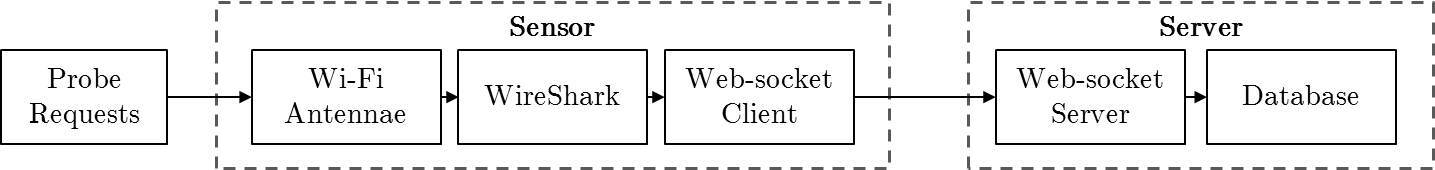
\includegraphics{images/pilot-study-system.jpeg}
  \caption{Schematic diagram showing the data collection process in the pilot study.}
  \label{figure:collection:pilot:schema}
\end{figure*}

The manual counting at these locations were done using a custom application \citet{bala2018}. The application was built for recording pedestrian footfall with precision and accuracy which was not possible when counted manually. The app records precise time stamp of every footfall with the precision of micro seconds which can be aggregated later at different time intervals. The code for the app is detailed in Section \ref{appendix:clicker}.

\subsection{Locations}

Five retail locations were chosen in consultation with the data partner for the pilot study keeping in mind their complexity and volume of footfall.
The sensors were installed at the locations in a phased manner and multiple manual counts were conducted at each location for 30 minute intervals.
The locations and their descriptions are summarised in Table \ref{table:collection:pilot:locations}.

\begin{figure*}
  \centering
  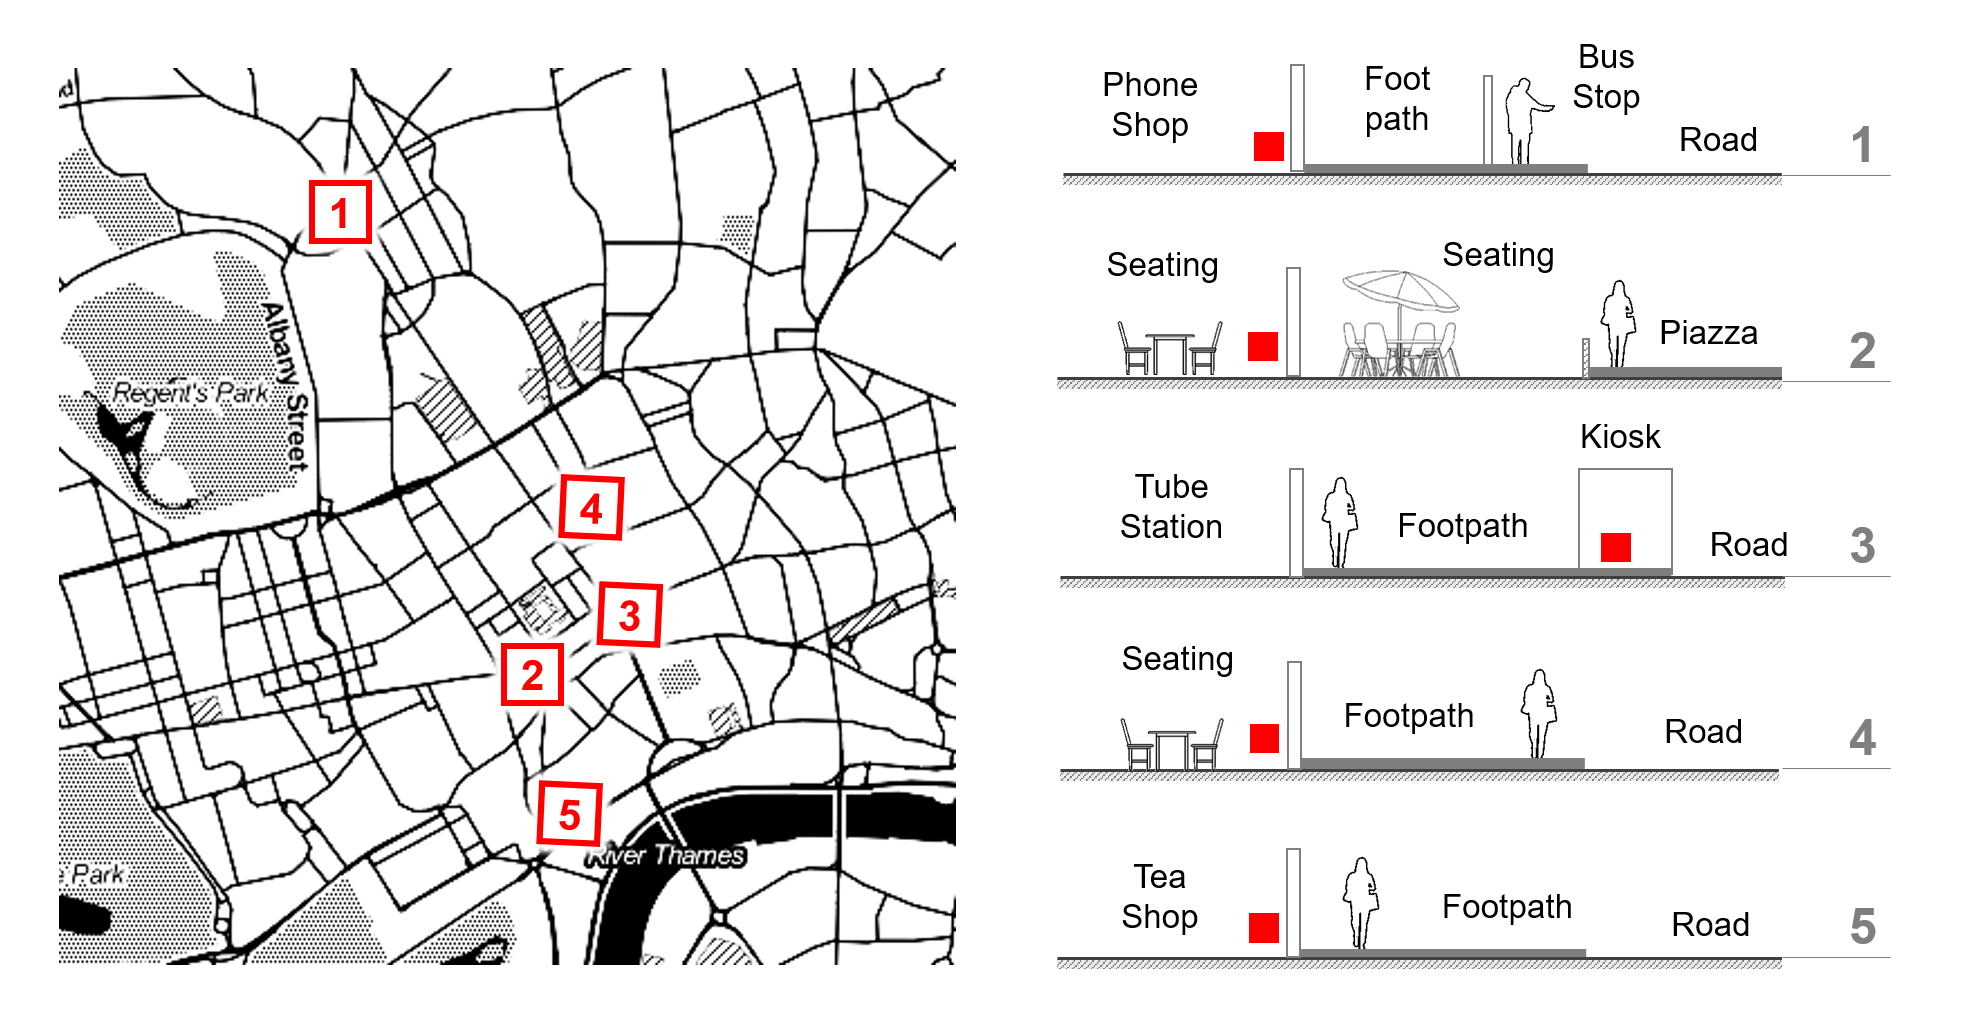
\includegraphics[trim={20 20 20 20},clip, width=\textwidth]{images/pilot-study-locations.png}
  \caption{Pilot study locations in London along with their corresponding sensor installation configurations.}
  \label{figure:collection:pilot:locations}
\end{figure*}

\begin{itemize}
  \item \textit{Location 1} is at the Camden high street in front of a mobile shop behind a bus stop. This location was chosen specifically because of the large amount of dwelling population at the bus stop and the stationary mobile devices inside the shop which is expected to create a large amount of noise along with the high footfall in the high street. The challenge here is to isolate the footfall from two sources of noises which are at equal distance from the sensor.
  \item \textit{Location 2} is at a square with a very low footfall but has a large amount of seating of the restaurant all around it. The challenge here is similar to that of the previous location but just that the volume of footfall is low which makes it one of the hardest locations for accurately estimating footfall.
  \item \textit{Location 3} is in front of Holborn station entrance in an information kiosk. This location was chosen for the really high volume from the station which is expected to cause noise. The challenge here is to be able to isolate the crowd inside the station from the footfall in the pavement.
  \item \textit{Location 4} is at a fast-food restaurant at a shopping center. The sensor has restaurant seating at one side and a pedestrian footfall at the other. The challenge here is that the stationary noise and the footfall are equidistant from the sensor.
  \item \textit{Location 5} is at the frontage of a shop at Strand with a mobile shop next door. This is the `cleanest' locations of all with only one clear source of noise which is at different distance from the footfall.
\end{itemize}

\begin{figure*}
  
\includegraphics{images/pilot-study-schedule.png}
  \caption{Outline of the `Medium data toolkit' devised to collect, process, visualise and manage the Wi-Fi probe requests data}
  \label{figure:collection:pilot:schedule}
\end{figure*}

The sensors were operational through out February and March, while manual counts were conducted in these locations in half hour sessions on at least two different days.
The schedule of the data collection and the days at which the manual counting were done are shown in Figure \ref{figure:collection:pilot:schedule}.

The survey was conducted for almost 2.5 months and about 33.5 million records were recorded which takes up to 1.8 GB of space on disk when encoded as text.
During the manual counts around 10,000 people were counted walking past these sensors.
A detailed account of the volume and velocity of data collected at these locations were given in Table \ref{table:collection:pilot:locations}.
The dataset collected was used extensively to develop and test the signal strength based filtering and sequence number based clustering methodology which are detailed in the Section \ref{section:device-fingerprinting}.

\begin{table} \footnotesize
\begin{center} \begin{tabular}{clllrr} \toprule
Id & Location & Type & Installation notes & Probes\textsuperscript{*} & Footfall\textsuperscript{**}\\
\midrule \addlinespace[0.2cm]
1 & Camden St.    & Phone Shop  & Bus stop in front         & 9.9 (297) & 3683 (33)\\ \addlinespace[0.1cm]
2 & St.Giles      & Restaurant  & Seating on both sides     & 3.9 (169) & 0346 (05)\\ \addlinespace[0.1cm]
3 & Holborn Stn.  & Info. Kiosk & Front of station entrance & 4.3 (303) & 2956 (46)\\ \addlinespace[0.1cm]
4 & Brunswick     & Fast Food   & Seating  on one side      & 3.4 (210) & 0960 (12)\\ \addlinespace[0.1cm]
5 & The Strand    & Tea Shop    & Phone shop next door      & 8.4 (382) & 1969 (21)\\ \addlinespace[0.05cm]
\bottomrule \end{tabular} \end{center}
\caption{Locations of data collection in the pilot study and the amount of data collected at each locations}
\label{table:collection:pilot:locations}
\end{table}
\marginnote[-1.5cm]{\textit{* Total probe requests in \(\times10^{6}\)(per minute)  ** Total footfall (per minute)}}
